\section{Domain Analysis}

\subsection{Objective of the Laboratory Work}

The objective of this laboratory work is to design, implement, and validate a dual-sensor temperature monitoring system on an Arduino Mega 2560 microcontroller. The system reads temperature data from two distinct sensor types --- an analog NTC thermistor and a digital DS18B20 --- and applies signal conditioning techniques to detect threshold crossings reliably. The application demonstrates the fundamental principles of sensor acquisition, analog-to-digital conversion, digital communication protocols, hysteresis-based threshold detection, and software debounce filtering in the context of embedded systems.

This laboratory work addresses several critical aspects of embedded sensor systems. First, it explores the differences between analog and digital temperature sensing, highlighting the trade-offs in accuracy, conversion time, interface complexity, and noise susceptibility. Second, it implements a complete signal processing pipeline --- from raw sensor data acquisition through conditioning and threshold evaluation to user-facing display and reporting. Third, the system uses FreeRTOS preemptive multitasking to separate the acquisition, conditioning, and display responsibilities into independent tasks with well-defined synchronization boundaries, demonstrating how real-time operating systems enable modular, responsive embedded applications.

The key learning objectives include understanding analog-to-digital conversion principles and the Steinhart-Hart equation for thermistor-based temperature measurement, mastering the OneWire digital communication protocol used by the DS18B20 sensor family, implementing hysteresis-based threshold detection to prevent alert oscillation near boundary values, applying software debounce filtering to validate the persistence of threshold crossings before triggering alerts, using FreeRTOS tasks with mutexes and binary semaphores for safe inter-task communication, and presenting processed sensor data through both an LCD display and a structured serial terminal interface.

\subsection{Problem Definition}

The task requires the development of a microcontroller-based temperature monitoring application with the following functional requirements. The system must periodically acquire temperature data from two sensors: one analog sensor (NTC thermistor) read via the built-in ADC, and one digital sensor (DS18B20) read via the OneWire protocol. The acquisition rate must be configurable, with a default period of 50 milliseconds to ensure responsive detection of temperature changes.

The acquired raw data must undergo signal conditioning through a threshold alerting module. This module implements hysteresis between two configurable values (for example, 28\textdegree C and 30\textdegree C) to prevent oscillation of the alert signal when the temperature hovers near the threshold boundary. Additionally, the module applies software debounce filtering that requires a configurable number of consecutive threshold crossings (for example, 5 readings) before confirming a state transition, ensuring that transient sensor noise or brief temperature spikes do not trigger false alerts.

The system must provide two output channels for displaying the monitoring results. An I2C LCD display shows the current temperature readings from both sensors and the alert status in a compact, human-readable format that alternates between information pages. Simultaneously, a structured report is printed to the serial terminal via STDIO (printf) at a lower frequency (every 2 seconds), providing detailed diagnostic information including raw ADC values, calculated resistance, converted temperatures, alert FSM states, debounce counters, threshold configuration, and cumulative statistics.

The application architecture must follow a modular design with clearly separated concerns. Sensor drivers, the threshold alert module, the LCD display driver, and the STDIO serial interface must each reside in reusable library modules under the PlatformIO project structure, while the lab-specific task orchestration resides in dedicated task files. The FreeRTOS scheduler manages three preemptive tasks: sensor acquisition (highest priority), signal conditioning with alerting (medium priority), and display with reporting (lowest priority).

Three LEDs provide immediate visual feedback on the system state: a green LED indicates normal operation (both sensors below threshold), a red LED lights when the analog sensor triggers an alert, and a yellow LED lights when the digital sensor triggers an alert. During debounce transitions, the corresponding LED blinks to indicate that a state change is being validated.

\subsection{Task Statement}

\begin{quote}
\textit{Sarcina de laborator --- Achiziție semnal binar}

\textit{Pentru un senzor analogic sau digital de temperatură, să se realizeze o aplicație pentru MCU care va achiziționa periodic semnalul de la senzorul selectat dintr-o listă de senzori, va afișa o alertă la depășirea unui prag prestabilit, afișând stările intermediare de condiționare și starea curentă în interfața STDIO, fie pe un display LCD, fie pe interfața serială.}

\textit{Varianta de realizare: implementarea unui sistem de monitorizare a doi senzori, unul analogic și unul digital, cu afișarea valorilor și alertelor de la ambii senzori pe display LCD.}
\end{quote}

\subsection{Used Technologies}

\subsubsection{Analog-to-Digital Conversion (ADC)}

Analog-to-Digital Conversion is the process of translating a continuous analog voltage signal into a discrete digital representation that a microcontroller can process. The Arduino Mega 2560 features a 10-bit successive approximation ADC with 16 multiplexed input channels. The 10-bit resolution means the ADC maps the input voltage range (0 V to 5 V by default) into 1024 discrete levels, yielding a resolution of approximately 4.88 mV per step.

The ADC conversion process begins when the firmware triggers a conversion on the selected channel. The successive approximation register (SAR) algorithm performs a binary search through the possible output codes, comparing the input voltage against an internally generated reference at each step. On the ATmega2560, the ADC clock is derived from the system clock through a prescaler, and a full conversion requires 13 ADC clock cycles (25 cycles for the first conversion after enabling the ADC). At the default prescaler setting of 128 (yielding a 125 kHz ADC clock from the 16 MHz system clock), a single conversion takes approximately 104 microseconds.

For temperature measurement with an NTC thermistor, the ADC reading represents the voltage at the midpoint of a resistive voltage divider formed by the thermistor and a fixed series resistor. The raw ADC value is then converted to resistance using the voltage divider equation, and subsequently to temperature using the Steinhart-Hart Beta parameter equation. This two-step conversion process introduces quantization noise from the ADC and component tolerance errors from the resistors, both of which must be considered when evaluating measurement accuracy.

The Steinhart-Hart Beta parameter equation used for NTC-to-temperature conversion is:

$$\frac{1}{T} = \frac{1}{T_0} + \frac{1}{B} \cdot \ln\left(\frac{R_{NTC}}{R_0}\right)$$

where $T$ is the absolute temperature in Kelvin, $T_0$ is the reference temperature (typically 298.15 K = 25\textdegree C), $B$ is the Beta coefficient of the thermistor (3950 K for the sensor used in this lab), $R_{NTC}$ is the measured thermistor resistance, and $R_0$ is the nominal resistance at $T_0$ (10 k$\Omega$). The resistance is calculated from the ADC reading using:

$$R_{NTC} = R_{series} \cdot \frac{ADC}{ADC_{max} - ADC}$$

where $R_{series}$ is the fixed series resistor (10 k$\Omega$), $ADC$ is the raw digital reading, and $ADC_{max}$ is the maximum ADC value (1023 for 10-bit resolution).

\subsubsection{OneWire Communication Protocol}

OneWire is a proprietary communication protocol developed by Dallas Semiconductor (now Maxim Integrated / Analog Devices) that enables bidirectional data exchange between a master device and one or more slave devices over a single data wire plus ground. The protocol is particularly significant in embedded temperature sensing because it allows the DS18B20 digital temperature sensor to communicate its readings using only one GPIO pin, minimizing the wiring complexity of multi-sensor installations.

The OneWire protocol operates at TTL voltage levels (typically 3.3 V or 5 V) and uses an open-drain bus topology with a pull-up resistor (typically 4.7 k$\Omega$) to VCC. Communication is initiated exclusively by the master, which drives the bus low to generate timing slots. The protocol defines several fundamental operations: Reset/Presence pulse (the master drives the bus low for at least 480 $\mu$s, then releases it; slave devices respond by pulling the bus low for 60--240 $\mu$s), Write Time Slot (the master drives the bus low and either releases it quickly for a logical `1' or holds it low for a logical `0'), and Read Time Slot (the master briefly drives the bus low, then samples the bus state; the slave holds the bus low for a `0' or releases it for a `1').

Each slave device on the OneWire bus has a unique 64-bit ROM code that serves as its address. The master can either address a specific device using the Match ROM command or communicate with all devices simultaneously using the Skip ROM command (useful when only one device is present). For temperature measurement, the master issues a Convert T command (0x44), which instructs the DS18B20 to begin its internal analog-to-digital conversion. The conversion time depends on the configured resolution: 93.75 ms at 9-bit, 187.5 ms at 10-bit, 375 ms at 11-bit, or 750 ms at 12-bit resolution. After conversion completes, the master reads the scratchpad memory containing the temperature result.

\subsubsection{I2C Communication Protocol}

Inter-Integrated Circuit (I2C) is a synchronous, multi-master, multi-slave serial communication protocol that uses two bidirectional open-drain lines: Serial Data (SDA) and Serial Clock (SCL). Developed by Philips Semiconductor (now NXP) in 1982, I2C has become one of the most widely used communication interfaces in embedded systems for connecting low-speed peripheral devices such as sensors, EEPROMs, real-time clocks, and LCD controllers.

\begin{figure}[H]
\centering
\IfFileExists{resources/DomainAnalysis/UsedTechnologies/i2c_protocol.png}{%
    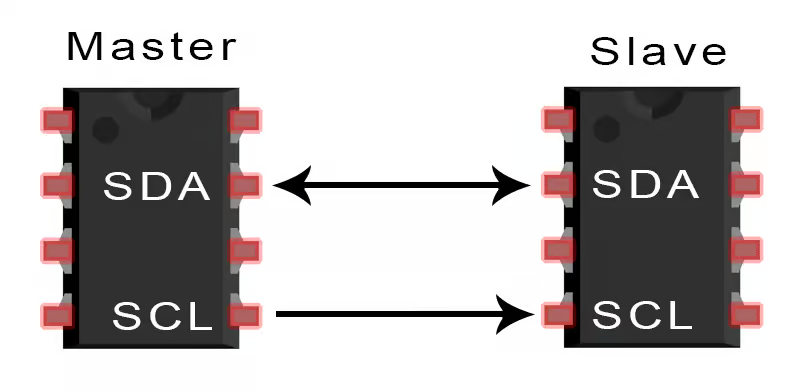
\includegraphics[width=0.7\textwidth]{resources/DomainAnalysis/UsedTechnologies/i2c_protocol.png}%
}{%
    \fbox{\parbox{0.68\textwidth}{\centering\color{gray}\small
        [Image pending --- save to resources/DomainAnalysis/UsedTechnologies/i2c\_protocol.png]}}%
}
\caption{I2C communication protocol timing diagram}
\label{fig:i2c_protocol}
\end{figure}

In this laboratory, I2C is used to communicate with the LCD 1602 display module through a PCF8574 I/O expander chip. The LCD module is configured at I2C address 0x27, and communication occurs at the standard 100 kHz clock speed. The Arduino Mega 2560 provides dedicated I2C pins: SDA on pin 20 and SCL on pin 21, both with internal pull-up capability. The I2C bus allows multiple devices to share the same two wires, making it possible to add additional sensors or displays without consuming additional GPIO pins.

Each I2C transaction follows a defined sequence: the master generates a START condition (SDA transitions from high to low while SCL is high), transmits the 7-bit slave address followed by a read/write bit, waits for an acknowledgment (ACK) from the addressed slave, transfers one or more data bytes (each followed by an ACK/NACK), and finally generates a STOP condition (SDA transitions from low to high while SCL is high). The LiquidCrystal\_I2C library abstracts these low-level protocol details, providing a simple API for text display operations.

\subsubsection{UART Serial Communication}

UART (Universal Asynchronous Receiver-Transmitter) is a hardware communication protocol for asynchronous serial data exchange between two devices. In this laboratory, UART is used to establish the STDIO communication channel between the Arduino Mega 2560 and the host PC, enabling structured diagnostic reports to be displayed in a terminal emulator.

The Arduino Mega 2560 provides four independent hardware UART ports (Serial, Serial1, Serial2, Serial3). UART0 (Serial) is connected to the on-board USB-to-serial converter, enabling seamless communication with the host PC at the configured baud rate of 9600 bits per second. The STDIO library redirection mechanism (implemented in the StdioSerial library module) maps the standard C I/O functions --- printf() for formatted output and fgets() for line input --- onto the UART hardware, allowing the application to use familiar C library functions instead of Arduino-specific Serial.print() calls.

\subsubsection{FreeRTOS Real-Time Operating System}

FreeRTOS is a real-time operating system (RTOS) kernel for embedded microcontrollers that provides preemptive multitasking, inter-task synchronization primitives, and deterministic scheduling. In this laboratory, FreeRTOS manages three concurrent tasks that together implement the sensor monitoring pipeline: acquisition, conditioning, and display/reporting.

The FreeRTOS scheduler uses a priority-based preemptive algorithm: at any given moment, the highest-priority task that is ready to run receives CPU time. When a higher-priority task becomes ready (for example, when a semaphore it was waiting on is given), the scheduler immediately preempts the running lower-priority task and switches context to the higher-priority one. This mechanism ensures that time-critical operations (such as sensor acquisition) are never delayed by lower-priority work (such as LCD display updates).

The synchronization primitives used in this lab include binary semaphores and mutexes. A binary semaphore acts as a lightweight signaling mechanism: the acquisition task \textit{gives} the semaphore after completing a reading cycle, and the conditioning task \textit{takes} the semaphore to wake up and process the new data. This event-driven approach eliminates the need for polling and minimizes CPU usage. A mutex (mutual exclusion semaphore) protects the shared data structures accessed by multiple tasks, ensuring that only one task can read or modify the shared state at any time. FreeRTOS mutexes provide priority inheritance: if a low-priority task holds the mutex and a high-priority task attempts to acquire it, the low-priority task temporarily inherits the higher priority, preventing the pathological condition known as priority inversion.

Task timing in FreeRTOS is managed through two mechanisms. The \texttt{vTaskDelayUntil()} function provides drift-free periodic execution by suspending the task until an absolute tick count is reached, compensating for any jitter in the task's execution time. The \texttt{xSemaphoreTake()} function with \texttt{portMAX\_DELAY} blocks the task indefinitely until the semaphore becomes available, providing efficient event-driven wake-up with zero polling overhead.

\subsubsection{Hysteresis-Based Threshold Detection}

Hysteresis is a signal conditioning technique that uses two distinct thresholds --- an upper (high) threshold and a lower (low) threshold --- to determine state transitions. Unlike single-threshold detection, which can produce rapid oscillation (chattering) when the signal hovers near the threshold value, hysteresis introduces a dead zone between the two thresholds where the system maintains its current state regardless of the input value.

In the context of temperature monitoring, hysteresis works as follows: the alert state activates when the temperature rises above the high threshold (e.g., 30\textdegree C) and deactivates only when the temperature drops below the low threshold (e.g., 28\textdegree C). If the temperature fluctuates between 28\textdegree C and 30\textdegree C, the alert state does not change --- it remains in whatever state it was previously in. This 2\textdegree C hysteresis band prevents the annoying and potentially harmful scenario where an alert repeatedly activates and deactivates due to minor temperature fluctuations around a single threshold.

The ThresholdAlert module in this lab extends basic hysteresis with software debounce filtering. Even with hysteresis, a sudden transient spike (caused by electrical noise, sensor glitches, or external interference) could momentarily push the reading above the threshold. The debounce mechanism requires $N$ consecutive readings (configurable, default 5) to confirm that the threshold has been genuinely crossed before committing to a state transition. If the reading drops back before $N$ confirmations are reached, the transition is cancelled and the system returns to its previous state. This two-layer protection (hysteresis + debounce) provides robust and reliable threshold detection suitable for industrial and safety-critical applications.

\subsubsection{Signal Conditioning Pipeline}

Signal conditioning in embedded sensor systems refers to the complete chain of operations applied to raw sensor data before it is presented to the user or used for decision-making. In this laboratory, the signal conditioning pipeline consists of several stages, each implemented as a distinct software module.

The first stage is raw data acquisition, where the ADC samples the NTC thermistor voltage and the OneWire interface reads the DS18B20 digital output. The second stage is physical quantity conversion, where the raw ADC value is transformed into a temperature reading through the Steinhart-Hart equation (for the analog sensor) or directly reported in degrees Celsius (for the digital sensor, which performs its own internal conversion). The third stage is threshold evaluation with hysteresis and debounce, where the converted temperature is compared against configurable thresholds to determine the alert state. The fourth and final stage is output formatting, where the processed data is presented on the LCD display and serial terminal in a human-readable format.

Each stage operates at its own temporal resolution: acquisition runs at 50 ms (20 Hz), conditioning is event-driven (triggered by each acquisition), and display/reporting runs at 500 ms (2 Hz) for the LCD and 2 seconds (0.5 Hz) for the STDIO report. This multi-rate architecture balances responsiveness (fast sensor reading) with resource efficiency (reduced LCD refresh and serial output overhead).

\subsection{Hardware Components}

\subsubsection{Arduino Mega 2560}

The Arduino Mega 2560 is the central microcontroller development board used in this laboratory. It is based on the ATmega2560 AVR microcontroller, which features a 16 MHz clock frequency, 256 KB of Flash program memory, 8 KB of SRAM, and 4 KB of EEPROM. The board provides 54 digital I/O pins (15 of which support PWM output), 16 analog input pins with 10-bit ADC resolution, 4 hardware UART serial ports, an SPI interface, and an I2C interface.

For this laboratory, the Arduino Mega 2560 serves multiple roles: it reads the analog NTC thermistor through its ADC (pin A0), communicates with the DS18B20 via a digital GPIO pin (pin 2) using the OneWire protocol, drives an I2C LCD display through its dedicated SDA/SCL pins (pins 20/21), controls three indicator LEDs through digital GPIO pins (pins 8, 9, 10), and runs the FreeRTOS scheduler to manage concurrent tasks. The board's generous memory (8 KB SRAM) is essential for running FreeRTOS with multiple tasks, each requiring its own stack allocation. The 256 KB Flash memory accommodates the application code, FreeRTOS kernel, sensor libraries, and the LCD display library without space constraints.

\begin{figure}[H]
\centering
\IfFileExists{resources/DomainAnalysis/HardwareComponents/arduino_mega_2560.png}{%
    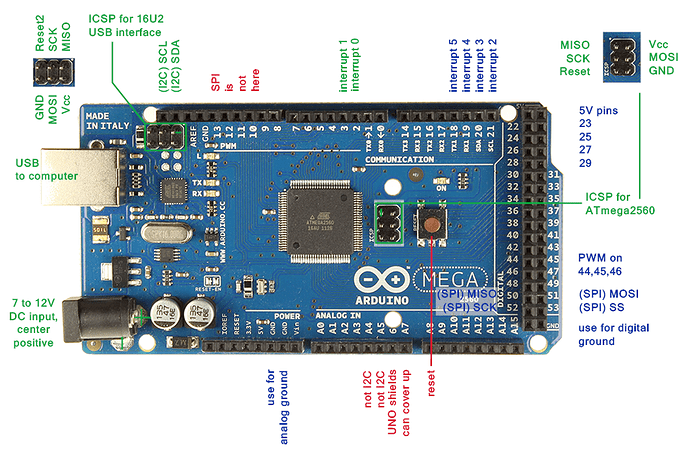
\includegraphics[width=0.65\textwidth]{resources/DomainAnalysis/HardwareComponents/arduino_mega_2560.png}%
}{%
    \fbox{\parbox{0.63\textwidth}{\centering\color{gray}\small
        [Photo pending --- save to resources/DomainAnalysis/HardwareComponents/arduino\_mega\_2560.png]}}%
}
\caption{Arduino Mega 2560 development board}
\label{fig:arduino_mega_2560}
\end{figure}

\subsubsection{NTC Thermistor (Analog Temperature Sensor)}

An NTC (Negative Temperature Coefficient) thermistor is a resistive temperature sensor whose electrical resistance decreases as temperature increases. The thermistor used in this laboratory has a nominal resistance of 10 k$\Omega$ at 25\textdegree C and a Beta coefficient ($B$ value) of 3950 K. These parameters define the resistance-temperature characteristic curve through the Steinhart-Hart Beta equation.

The NTC thermistor is connected in a voltage divider configuration with a 10 k$\Omega$ fixed series resistor. The midpoint voltage of this divider is fed to the Arduino's analog input pin A0. As the temperature changes, the thermistor resistance changes, altering the voltage division ratio and producing a corresponding change in the ADC reading. At 25\textdegree C, the thermistor resistance equals the series resistance (both 10 k$\Omega$), placing the divider midpoint at exactly VCC/2 = 2.5 V, which corresponds to an ADC reading of approximately 512 out of 1023. At higher temperatures, the thermistor resistance decreases, pulling the midpoint voltage lower and producing a smaller ADC reading. At lower temperatures, the resistance increases, pushing the voltage higher.

The NTC thermistor's advantages include its high sensitivity (large resistance change per degree), low cost, small physical size, and fast thermal response time. Its primary limitation is the nonlinear resistance-temperature relationship, which requires the Steinhart-Hart equation (or a lookup table) for accurate conversion. The 10-bit ADC resolution of the Arduino provides a theoretical temperature resolution of approximately 0.1\textdegree C near the 25\textdegree C nominal point, though practical accuracy is limited by component tolerances and electrical noise.

\begin{figure}[H]
\centering
\IfFileExists{resources/DomainAnalysis/HardwareComponents/ntc_thermistor.png}{%
    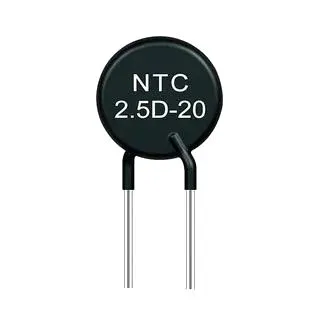
\includegraphics[width=0.4\textwidth]{resources/DomainAnalysis/HardwareComponents/ntc_thermistor.png}%
}{%
    \fbox{\parbox{0.38\textwidth}{\centering\color{gray}\small
        [Photo pending --- save to resources/DomainAnalysis/HardwareComponents/ntc\_thermistor.png]}}%
}
\caption{NTC thermistor (10K, Beta=3950)}
\label{fig:ntc_thermistor}
\end{figure}

\subsubsection{DS18B20 Digital Temperature Sensor}

The DS18B20 is a digital temperature sensor manufactured by Maxim Integrated (formerly Dallas Semiconductor) that provides 9-to-12-bit temperature measurements over a single-wire digital interface. Unlike the NTC thermistor, which outputs an analog voltage that must be externally converted, the DS18B20 performs its own internal analog-to-digital conversion and communicates the result digitally, eliminating analog noise and conversion errors in the communication path.

The DS18B20 measures temperatures from $-55$\textdegree C to $+125$\textdegree C with a configurable resolution. At 10-bit resolution (used in this lab), the sensor provides 0.25\textdegree C precision with a conversion time of approximately 187.5 ms. The sensor's accuracy is $\pm$0.5\textdegree C over the $-10$\textdegree C to $+85$\textdegree C range, making it suitable for most environmental monitoring applications.

Communication with the DS18B20 uses the OneWire protocol over a single data pin (DQ), plus power (VCC) and ground (GND). A 4.7 k$\Omega$ pull-up resistor on the DQ line is required because the OneWire bus uses an open-drain topology. Each DS18B20 has a factory-programmed unique 64-bit serial code that enables multiple sensors to share the same OneWire bus and be individually addressed. In this laboratory, only one DS18B20 is used, and the Skip ROM command is employed for simplified single-device communication.

The DS18B20's key advantages over the NTC thermistor include digital output (immune to analog noise on the communication path), factory-calibrated accuracy, direct temperature output without external conversion circuitry, addressable multi-sensor capability, and user-configurable resolution. However, it requires a more complex communication protocol (OneWire), has a longer conversion time compared to an ADC reading, and costs more than a simple thermistor.

\begin{figure}[H]
\centering
\IfFileExists{resources/DomainAnalysis/HardwareComponents/ds18b20.png}{%
    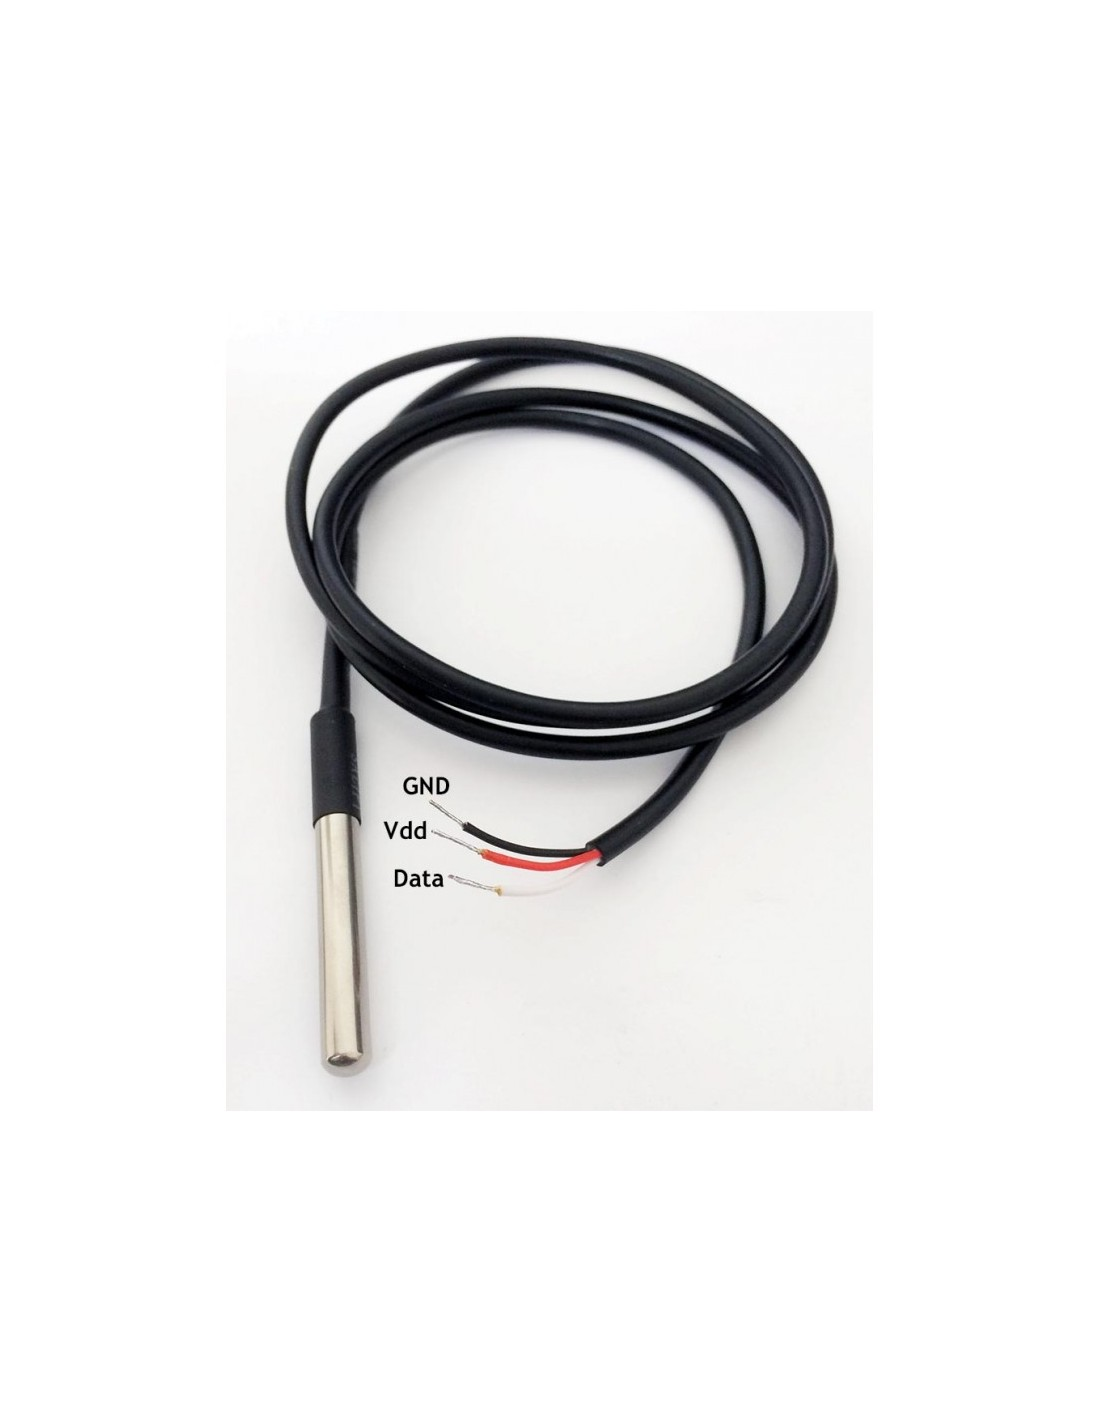
\includegraphics[width=0.4\textwidth]{resources/DomainAnalysis/HardwareComponents/ds18b20.png}%
}{%
    \fbox{\parbox{0.38\textwidth}{\centering\color{gray}\small
        [Photo pending --- save to resources/DomainAnalysis/HardwareComponents/ds18b20.png]}}%
}
\caption{DS18B20 digital temperature sensor (TO-92 package)}
\label{fig:ds18b20}
\end{figure}

\subsubsection{LCD 1602 with I2C Interface}

The LCD 1602 is a character liquid crystal display module capable of showing 16 characters per line across 2 lines. When equipped with a PCF8574-based I2C backpack module, the display communicates with the microcontroller over just two wires (SDA and SCL) instead of requiring 6--10 parallel data pins. The I2C address is typically 0x27, though some modules use 0x3F depending on the address jumper configuration.

In this laboratory, the LCD serves as the primary real-time display for temperature readings and alert status. The display alternates between two information pages every 2 seconds: the first page shows the current analog and digital temperatures along with the overall system status (OK, ALERT: Analog, ALERT: Digital, or ALERT: A+D), while the second page displays the configured threshold values for reference. The 16-character line width constrains the information density, requiring careful formatting to present the most relevant data in a compact form.

\begin{figure}[H]
\centering
\IfFileExists{resources/DomainAnalysis/HardwareComponents/lcd_1602_i2c.png}{%
    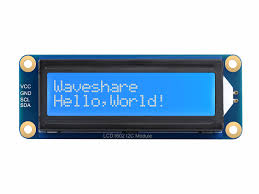
\includegraphics[width=0.5\textwidth]{resources/DomainAnalysis/HardwareComponents/lcd_1602_i2c.png}%
}{%
    \fbox{\parbox{0.48\textwidth}{\centering\color{gray}\small
        [Photo pending --- save to resources/DomainAnalysis/HardwareComponents/lcd\_1602\_i2c.png]}}%
}
\caption{LCD 1602 display with I2C backpack module}
\label{fig:lcd_1602_i2c}
\end{figure}

\subsubsection{LEDs with Current-Limiting Resistors}

Three LEDs provide immediate visual feedback on the system state. Each LED is connected to a digital GPIO pin through a 220~$\Omega$ current-limiting resistor, which restricts the forward current to approximately 15 mA at the 5 V logic level (accounting for the typical 2 V forward voltage drop across the LED). The three colors encode the following system states:

The green LED (pin 8) indicates normal system operation, meaning both sensors are reading below their respective thresholds. The red LED (pin 9) indicates that the analog sensor (NTC thermistor) has triggered a threshold alert. The yellow LED (pin 10) indicates that the digital sensor (DS18B20) has triggered a threshold alert. During debounce transitions (when the system is counting consecutive confirmations), the corresponding LED blinks to provide a visual cue that a state change is being validated but not yet confirmed. When any alert is active, the green LED turns off to provide unambiguous status indication.

\begin{figure}[H]
\centering
\IfFileExists{resources/DomainAnalysis/HardwareComponents/led.png}{%
    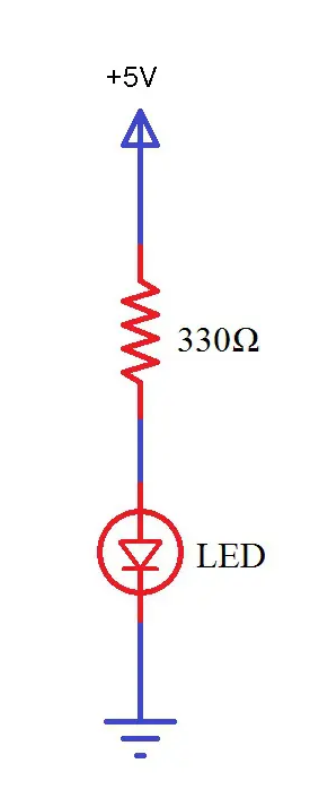
\includegraphics[width=0.35\textwidth]{resources/DomainAnalysis/HardwareComponents/led.png}%
}{%
    \fbox{\parbox{0.33\textwidth}{\centering\color{gray}\small
        [Photo pending --- save to resources/DomainAnalysis/HardwareComponents/led.png]}}%
}
\caption{Standard 5mm LEDs (green, red, yellow)}
\label{fig:led}
\end{figure}

\subsubsection{Resistors}

Several resistors are used in the circuit. A 10 k$\Omega$ resistor forms the upper half of the voltage divider for the NTC thermistor, creating a known reference against which the thermistor's variable resistance produces a measurable voltage. A 4.7 k$\Omega$ pull-up resistor on the DS18B20 data line provides the required pull-up voltage for the open-drain OneWire bus. Three 220 $\Omega$ resistors limit the current through the indicator LEDs to safe operating levels.

\subsection{Software Components}

\subsubsection{PlatformIO}

PlatformIO is a professional open-source ecosystem for embedded development that integrates with Visual Studio Code as an extension. It provides comprehensive project management, automatic library dependency resolution, multi-board and multi-environment support, and unified build/upload/monitor tools. In this laboratory, PlatformIO manages the compilation environment for the Arduino Mega 2560, automatically resolves library dependencies (FreeRTOS, OneWire, DallasTemperature, LiquidCrystal\_I2C), and provides the serial monitor for observing STDIO output.

The PlatformIO project configuration (\texttt{platformio.ini}) defines a dedicated environment for Lab 3.1 with the required build flags and library dependencies, enabling the project to maintain multiple lab configurations simultaneously without code conflicts whether to run one lab environment or another.

\begin{figure}[H]
\centering
\IfFileExists{resources/DomainAnalysis/SoftwareComponents/platformio.png}{%
    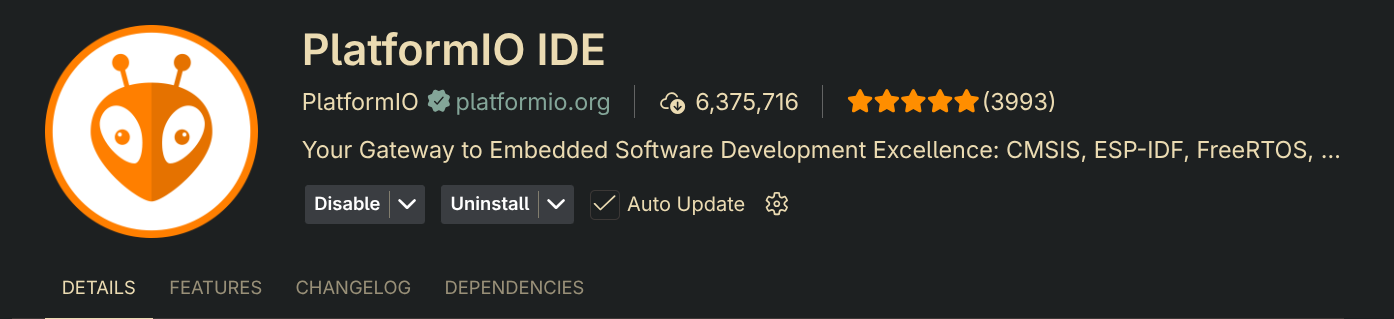
\includegraphics[width=0.75\textwidth]{resources/DomainAnalysis/SoftwareComponents/platformio.png}%
}{%
    \fbox{\parbox{0.73\textwidth}{\centering\color{gray}\small
        [Screenshot pending --- save to resources/DomainAnalysis/SoftwareComponents/platformio.png]}}%
}
\caption{PlatformIO IDE in VS Code with Lab 3.1 project}
\label{fig:platformio}
\end{figure}

\subsubsection{Wokwi Simulator}

Wokwi is an embedded systems simulator available both as a web application and as a VS Code extension. It supports Arduino, ESP32, Raspberry Pi Pico, and other popular platforms, providing virtual components including LEDs, buttons, LCDs, temperature sensors (NTC thermistors and DS18B20), and serial terminals. Wokwi enables testing of the complete application in a simulated environment before deploying to physical hardware, which is particularly valuable for temperature sensor applications where controlled temperature variation would otherwise require physical heating/cooling equipment.

In this laboratory, Wokwi simulates the complete circuit: the Arduino Mega 2560, an NTC thermistor with adjustable temperature, a DS18B20 sensor with adjustable temperature, a 16x2 I2C LCD display, three LEDs with resistors, and the voltage divider and pull-up resistors. The simulator allows interactive temperature adjustment during runtime, making it possible to test threshold crossings, hysteresis behavior, and debounce filtering without physical sensor manipulation.

\begin{figure}[H]
\centering
\IfFileExists{resources/DomainAnalysis/SoftwareComponents/wokwi.png}{%
    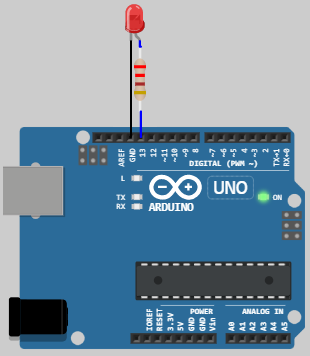
\includegraphics[width=0.75\textwidth]{resources/DomainAnalysis/SoftwareComponents/wokwi.png}%
}{%
    \fbox{\parbox{0.73\textwidth}{\centering\color{gray}\small
        [Screenshot pending --- save to resources/DomainAnalysis/SoftwareComponents/wokwi.png]}}%
}
\caption{Wokwi simulator running the Lab 3.1 circuit}
\label{fig:wokwi}
\end{figure}

\subsection{Case Study: Industrial Temperature Monitoring Systems}

The dual-sensor temperature monitoring architecture implemented in this laboratory closely mirrors industrial temperature monitoring systems used in manufacturing, food processing, HVAC, and data center environments. In these real-world applications, redundant sensor configurations (combining analog and digital sensors) provide both measurement diversity and fault tolerance.

In pharmaceutical cold chain monitoring, for example, regulatory requirements mandate continuous temperature logging with alarm capabilities. Pharmaceutical storage facilities use multiple temperature sensors per zone, with hysteresis-based alerting to prevent nuisance alarms during door openings while ensuring that sustained temperature excursions trigger immediate notifications. The signal conditioning pipeline implemented in this lab --- acquisition, threshold evaluation with hysteresis, debounce filtering, and multi-channel reporting --- directly corresponds to the processing stages found in commercial pharmaceutical monitoring systems, albeit at a smaller scale.

Data center thermal management represents another relevant application. Server rooms require precise environmental monitoring to prevent equipment overheating while avoiding unnecessary cooling that increases energy costs. Modern data center monitoring systems deploy hundreds of temperature sensors (both thermistors for air temperature and digital sensors integrated into server motherboards), process their readings through configurable threshold engines, and generate alerts through dashboards and notification systems. The FreeRTOS-based task architecture used in this lab demonstrates the same separation of concerns found in these larger systems: dedicated acquisition tasks for sensor polling, middleware conditioning tasks for threshold logic, and presentation tasks for human-machine interface updates.

The hysteresis technique implemented in the ThresholdAlert module is particularly important in automotive Engine Control Units (ECUs), where coolant temperature monitoring must balance sensitivity (detecting genuine overheating conditions rapidly) with stability (avoiding false alarms during normal thermal cycling). Automotive ECUs typically employ 2--5\textdegree C hysteresis bands with multi-sample debounce windows, closely matching the approach used in this laboratory.
